The central feature of the Compact Muon Solenoid is a superconducting solenoid magnet with a 6m internal diameter, providing an internal magnetic field of 3.8 T - it is the most powerful solenoid magnet on earth. An image of the solenoid magnet placed within the CMS detector is shown in Figure \ref{fig:Magnet}.

\begin{figure}[H]
    \centering
    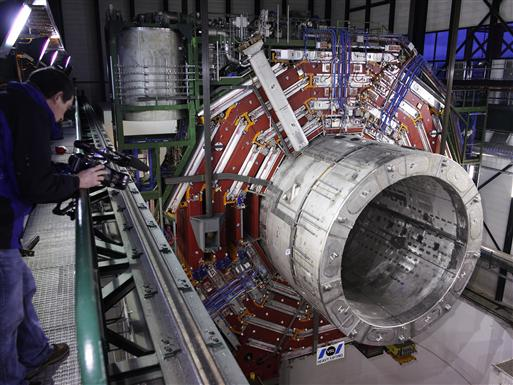
\includegraphics[width=0.7\textwidth]{Images/CMS/Magnet/CMS_Solenoid_Magnet.jpg}    
    \caption{The in-progress CMS detector, with the central solenoid magnet visible.}
    \label{fig:Magnet}
\end{figure}

The CMS solenoid magnet plays the dual purpose of producing a magnetic field both in the inner and outer detector, in the outer detector thanks to the ferromagnetic material composition of the CMS outer steel flux return yokes, while also acting as the main support unit to sustain the massive weight of CMS. The magnetic field strength across the inner and outer detector are shown in Figure \ref{fig:MagneticField}. 

\begin{figure}[H]
    \centering
    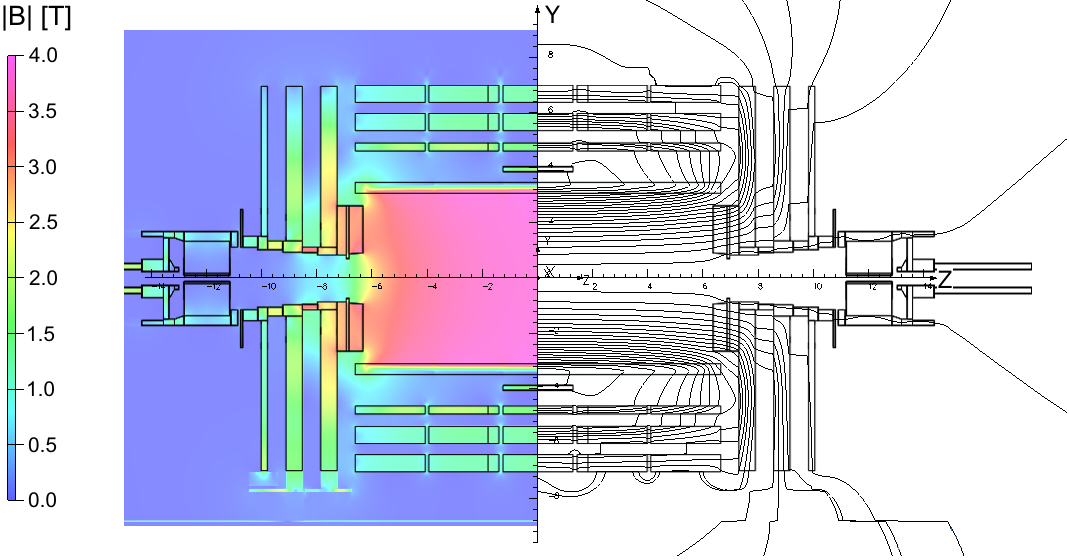
\includegraphics[width=0.7\textwidth]{Images/CMS/Magnet/CMS_Magnetic_Field.png}    
    \caption{CMS magnetic field produced by the solenoid magnetic and steel flux return yoke.}
    \label{fig:MagneticField}
\end{figure}

Having a strong magnetic field in the inner tracker region is crucial for the measurements of charged particle tracks and momentum measurement. Additionally, because particles produced in LHC collisions are moving near the speed of light as they traverse the CMS tracker, they spend a finite amount of time in the tracker region, and the stronger the magnetic field in the region the more likely the particle can be ``bent" allowing the a high transverse momentum measurement. In particular, the presence of a strong magnetic field to measure the tracks of high \pt particles is of high interest as these particles are more likely to have come from interesting hard interactions, such as those producing a massive particle. 

A magnetic field is also produced in the outer CMS detector, which is crucial for the measurement of muon tracks by the CMS muon system.